\documentclass[12pt]{article}

\usepackage{polski}
\usepackage[utf8]{inputenc}
\usepackage{graphicx}
\usepackage{tikz}
\usepackage{amsmath}
\usepackage{epstopdf}
\usepackage{float} 
%\usepackage[colorlinks=true]{hyperref}
%\usepackage[all]{hypcap}
%\usepackage{showframe}
\usepackage{geometry}
 \geometry{
 a4paper, 
 left=30mm,
 right=30mm,
 top=30mm,
 bottom=30mm,
 }
 
\begin{document}

\section{Wyniki pomiarów i aproksymacji}

\subsection{Charakterystyka napięciowo-częstotliwościowa \\ falownika NT-110}

W celu zachowania zdolności momentowej silnika prądu przemiennego, przy
zasilaniu falownikowym postuluje się stałość stosunku napięcia zasilającego
silnik do jego częstotliwości.

Ponieważ $T= \frac{P}{\omega}$ oraz:

\begin{equation*}
	\begin{cases}
		P \sim U^2 \\
		P \sim \frac{1}{\omega}
	\end{cases}
\end{equation*}

stąd wynika, iż $T \sim \frac{U^2}{\omega^2}$, co jest równoważne z $T \sim
\left(\frac{U}{f}\right)^2$, więc aby $T=\text{const}$ musi być spełniony
warunek $\frac{U}{f} = \text{const}$

\begin{figure}[!htb]
	\begin{center}
		\includegraphics[trim=5cm 9cm 5cm 9cm]{../res/img/U_f(f).pdf} 
	\end{center}
	\caption{Charakterystyka $U=f(f)$ falownika}
\end{figure}

Linią przerywaną na charakterystykę naniesiona jest aproksymacja jej liniowej
części. Jest ona dana wzorem $U=6.85f+59.64$. Stosunek $\frac{U}{f}$ nie jest
więc stały. Stały jest natomiast stosunek $\frac{U-59.64}{f}$, jest to zapewne
celowy zabieg producenta falownika.

\newpage

\subsection{Charakterystyki mechaniczne silnika SG-100-L4B}

Parametry nominalne tego silnika to $P_n=3[kW]$, $U_n=220/380[V]$,
$I_n=12/6.9[A]$, $n_n=1415[\frac{obr}{min}]$.
Zdjęte fragmenty charakterystyk wyglądają następująco:

\begin{figure}[!htb]
	\begin{center}
		\includegraphics[trim=5cm 9cm 5cm 9cm]{../res/img/T_f(n)2.pdf} 
	\end{center}
	\caption{Charakterystyki mechaniczne $T=f(n)$ silnika}
\end{figure}

Są to końcowe fragmenty charakterystyk położone za prędkością obrotową
krytyczną, czyli w obszarze normalnej pracy silnika.

\newpage

\subsection{Przełącznik gwiazda-trójkąt}

Rozruch silnika trójfazowego z uzwojeniami połączonymi w trójkąt wiąże się z
bardzo dużym udarem prądowym, szczególnie gdy silnik jest już przed
uruchomieniem obciążony na wale. Przy połączeniu silnika w gwiazdę prąd
rozruchowy jest około 3 razy mniejszy, dlatego do rozruchu stosuje się
przełączniki gwiazda-trójkąt, które uruchamiają silnik przy połączeniu uzwojeń w
gwiazdę po czym po osiągnięciu nominalnej prędkości obrotowej uzwojenia silnika
przełączane są w trójkąt. Prądy udarowe są wtedy znacznie mniejsze.

\begin{figure}[!htb]
	\begin{center}
		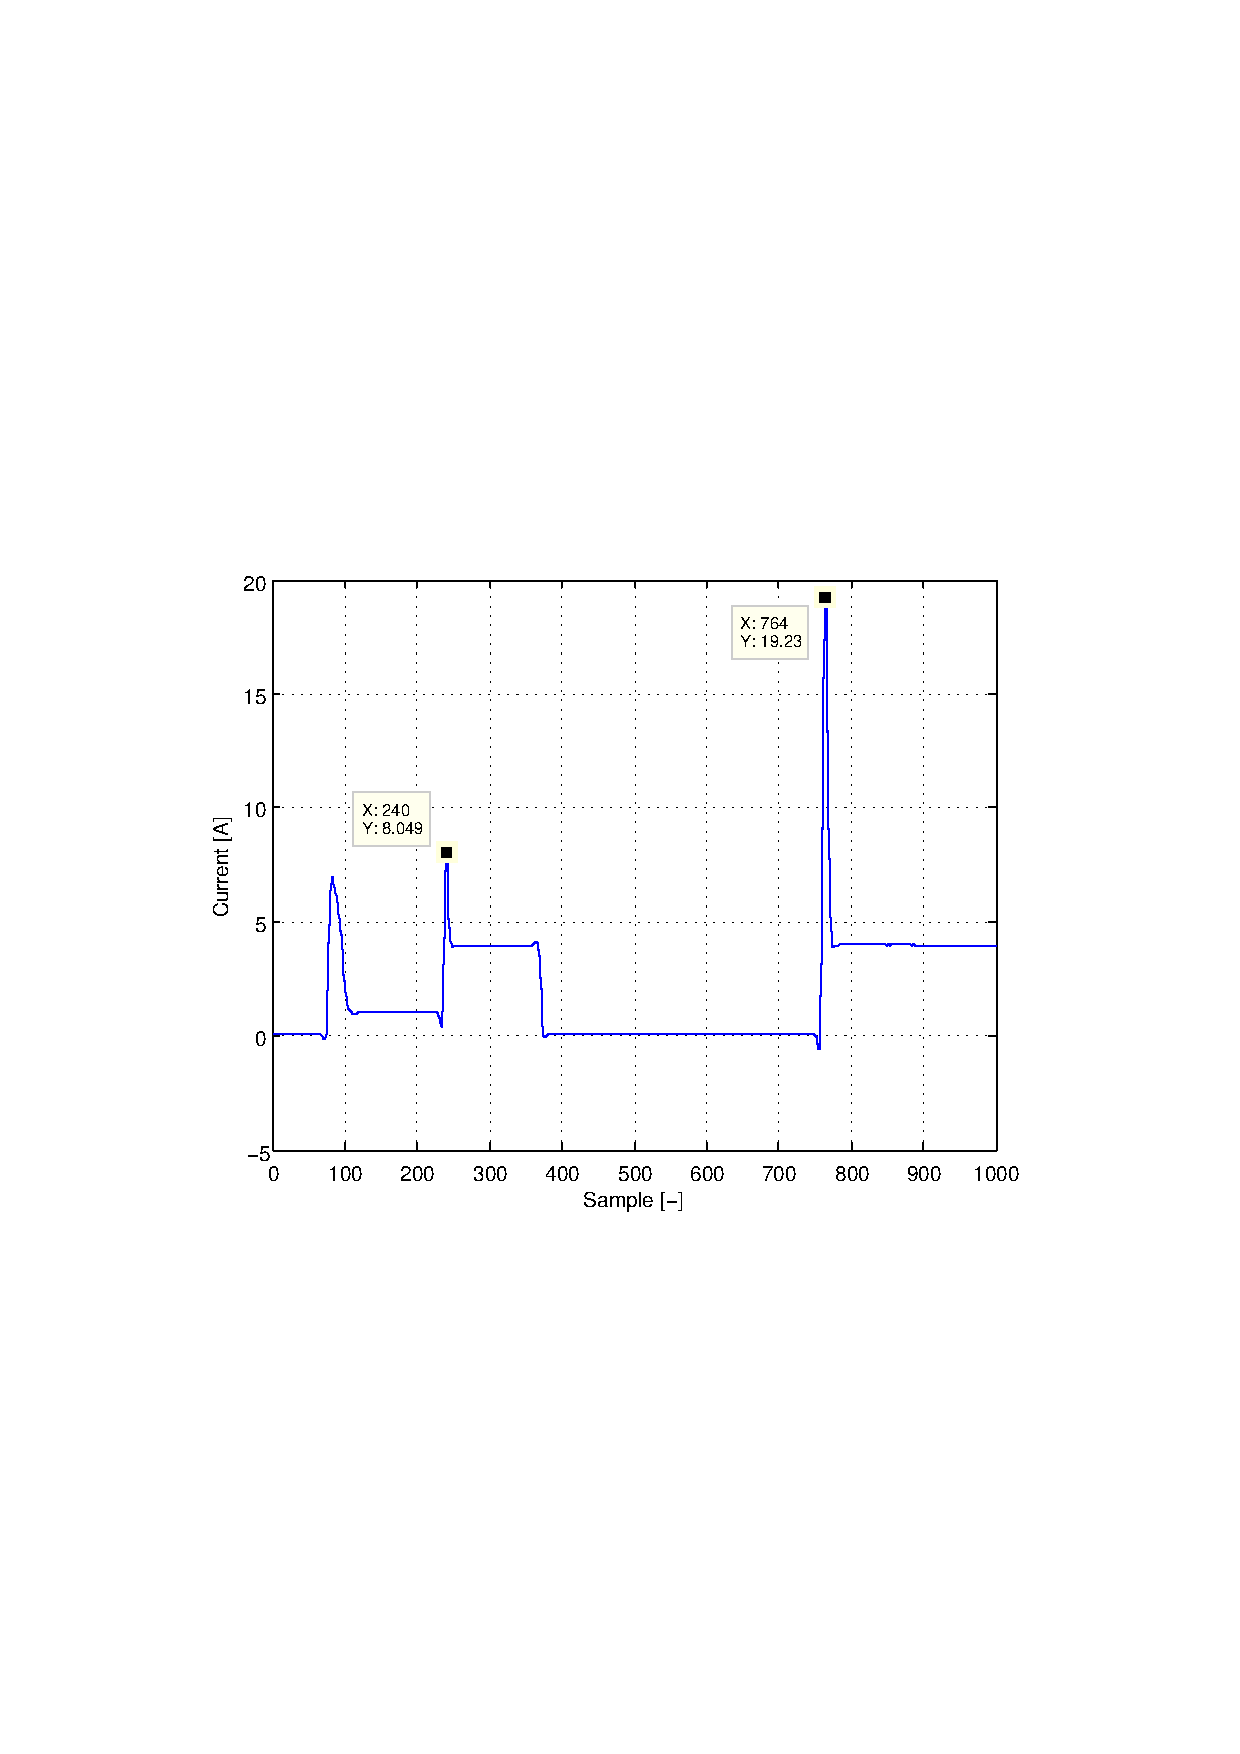
\includegraphics[trim=5cm 9cm 5cm 9cm]{../res/img/Ir.pdf}  
	\end{center}
	\caption{Przebieg prądu stojana silnika podczas rozruchu, dla przełącznika
	gwiazda-trójkąt, oraz podczas uruchomienia silnika w konfiguracji trójkąta}
\end{figure}

Szczytowy prąd rozruchowy przy zastosowaniu przełącznika jest w przybliżeniu
2.39 raza mniejszy niż podczas uruchomienia silnika od razu w konfiguracji
gwiazdowej. Jest to znaczny spadek strat mocy podczas rozruchu silnika.

\newpage

\subsection{Wyznaczenie parametrów schematu zastępczego \\ ($R_r'$, $R_s$,
$X_k$) w oparciu o aproksymację komputerową}

W trakcie wykonania ćwiczenia zdjęta została charakterystyka $T=f(s)$ silnika
indukcyjnego. Niestety zebrane punkty nie zgadzają się z teoretycznym
przebiegiem charakterystyki. Dodatkowo z nieznanych przyczyn były one zdjęte
przez program pomiarowy w kolejności niemonotonicznej, co pozwala przypuszczać,
że wyniki aproksymacji nie będą poprawne. W celu dopasowania punktów pomiarowych
do teoretycznego przebiegu charakterystyki pominąłem kilka punktów dla
największego poślizgu, ponieważ zmierzony dla nich moment był ujemny, co nie
jest możliwe. Wykonana aproksymacja dla pozostałych punktów przedstawia się
następująco:

\begin{figure}[!htb]
	\begin{center}
		\includegraphics[trim=5cm 9cm 5cm 9cm]{../res/img/T_f(s)3.pdf}  
	\end{center}
	\caption{Charakterystyka momentu silnika w funkcji poślizgu $T=f(s)$, dla pracy
	silnikowej i prądnicowej}
\end{figure}

Aproksymata została wyznaczona dla parametrów $U_s=400[V]$, $p=3$, $c_s=0.95$,
$\omega_0=314[\frac{rad}{s}]$.

Teoretyczny przebieg charakterystyki dany jest wzorem:

\begin{equation*}
	T(s) = \frac{pU_s^2c_s^2}{\omega_0}\cdot
	\frac{R_r's}{(R_r'+sc_sR_s)^2+(sX_k)^2}
\end{equation*}
 
Parametry zastępcze są więc równe $R_r'=19.05[\Omega]$, $R_s=44.93[\Omega]$,
$X_k=62.05[\Omega]$.

\section{Wnioski}

Ćwiczenie pozwoliło zapoznać się z obsługą falownikowego sterowania silnikiem
indukcyjnym. Jak widać z przeprowadzonych pomiarów, amplituda napięcia
wyjściowego falownika nie jest stała, lecz liniowo zależy od jego
częstotliwości, co ma na celu zachowanie zdolności momentowych silnika w
szerokim zakresie częstotliwości jego zasilania.

W przypadku braku dostępnego zasilania falownikowego problemem staje się rozruch
silników dużej mocy, ponieważ chcąc wykorzystać pełną jego moc, uzwojenia
silnika łączone są w trójkąt. Niestety taka konfiguracja oprócz zwiększonych
mocy osiągalnych powoduje również trzykrotny wzrost prądów, zarówno pracy jak i
rozruchowych. Ponieważ moc strat zależy od kwadratu prądu płynącego przez
uzwojenia, celowe jest ograniczenie za wszelką cenę prądów rozruchowych silnika.
W tym celu stosuje się uruchamianie silnika w konfiguracji gwiazdowej, a
następnie po osiągnięciu nominalnej prędkości obrotowej przełączenie do
konfiguracji pracy. Jak wynika z przeprowadzonych pomiarów istotnie szczytowy
prąd rozruchowy był znacznie mniejszy niż przy bezpośrednim uruchomieniu silnika
w konfiguracji trójkąta.

Ostatnim przeprowadzonym badaniem był pomiar momentu silnika w funkcji jego
poślizgu. Niestety z nieznanych przyczyn uzyskane punkty pomiarowe nie są w
pełni zgodne z teoretycznym przebiegiem tej krzywej. Dlatego wyznaczona
aproksymacja nie może być brana pod uwagę jako rzetelne źródło wyznaczonych
parametrów zastępczych silnika. Charakterystyka została aproksymowana dla
punktów pomiarowych z odrzuceniem tych które okazują się być niezgodne z
teoretycznym jej przebiegiem.




\end{document}
